\documentclass[a4paper]{article}

\usepackage[french]{babel}
\usepackage[T1]{fontenc}
\usepackage[utf8]{inputenc}
\usepackage{amsmath}
\usepackage{graphicx}
\usepackage{lmodern}
\usepackage[left=3cm, right=3cm, bottom=4cm, top=4cm]{geometry}
\usepackage{array}
\usepackage{pdfpages}

\usepackage{hyperref}
\hypersetup{
    colorlinks,
    citecolor=black,
    filecolor=black,
    linkcolor=black,
    urlcolor=black
}

\title{Rapport de pré-étude}

\author
{
	Pierre-Marie {\sc Airiau}\\
    Valentin {\sc Esmieu}\\
    Hoel {\sc Kervadec}\\
    Maud {\sc Leray}\\
    Florent {\sc Mallard}\\
    Corentin {\sc Nicole}
}

\date{\today}

\newcommand{\pagevierge}[0]{\newpage\thispagestyle{empty}\null\newpage}

\begin{document}
    % Ouh c'est sale.
    \hypersetup{pageanchor=false}
    
\includepdf[pages=1]{figure/couv.pdf}
    \hypersetup{pageanchor=true}
    
    \newpage
    \thispagestyle{empty}
    \mbox{}
    
    \newpage
    % A decommenter pour la release
    \setcounter{tocdepth}{2}
    \tableofcontents
    \setlength{\parskip}{10pt}
    
    \newpage
    \thispagestyle{empty}
    \mbox{}
    
    \newpage
    \section{Introduction}
	La sécurisation des systèmes est une problématique majeure de la société moderne. En ce sens, de nombreuses méthodologies ont été développées~\cite{introSecurite,ADTreeKordy} dans le but d'identifier les risques et de les quantifier. C'est avec cet objectif que le concept d'arbres d'attaque et de défense (ADTrees) a vu le jour.

	Lors de la phase de pré-étude, nous avons pu comprendre l’intérêt pratique de la construction des ADTrees. Leur utilisation permet d'identifier de manière précise les différentes attaques possibles contre un système et de les valuer en termes de coût, de probabilité, etc. ADTool~\cite{adtool_paper} (Attack-Defense Tree Tool), un logiciel libre développé pour l'implémentation de ces arbres sur support informatique, a été mis à disposition pour ce projet. Lors de sa prise en main, des limites ont été constatées. En effet, dans un cas concret d'expertise en sécurité, le système doit faire face à une multitude d'attaques possibles et, par conséquent, l'ADTree qui les modélisera sera de très grande taille. Dans ce cas, il est très difficile pour l'expert d'en extraire des informations pertinentes au premier coup d’œil. Or, ADTool ne fournit pas d'outil permettant à l'utilisateur de simplifier l'analyse de l'arbre. 

	L'objectif de ce projet est donc la création d'un logiciel intégrant ADTool et permettant de faciliter le travail d'un expert en sécurité, en lui fournissant des outils pour analyser facilement ses ADTrees. Ce logiciel portera le nom de \glasir{}  (prononcé [\textipa{glaziK}]). Il s'agit du nom d'un arbre aux feuilles d'or dans la mythologie nordique~\cite{vikingCulture}.

	Ce rapport présente les spécifications fonctionnelles de \glasir{}. Tout d'abord, les limites d'ADTool seront abordées, afin de justifier l'intérêt de \glasir{}. Puis nous détaillerons les différentes fonctionnalités destinées à l'analyse des ADTrees. Enfin, quelques améliorations supplémentaires seront également précisées pour offrir un meilleur confort de création et édition d'arbres. Ces spécifications seront faites en prenant en exemple une situation précise : celle d'un expert en sécurité chargé par le Service des Transports en commun de l'Agglomération Rennaise (STAR) de déterminer les failles de leurs systèmes de paiement.
    
    \chapter{Contexte}

	\section{Un contexte mondial}

	Le bon fonctionnement des transports en commun dépend de nombreux facteurs. Qu'il soit humain, ou bien technique, le moindre dysfonctionnement impactera le système entier très rapidement. Ainsi, un simple tour d'horizon de la presse internationale fait vite remonter à la surface de nombreux cas de paralysie des transports publics urbains dans le monde entier.

		\subsection{ Les risques d'atteinte aux passagers }

	Parmi tous les cas de paralysie, les plus marquants à l'échelle internationale sont ceux impliquant des dégâts humains importants parmi les passagers. Il s'agit, dans la plupart des cas, d'attaques terroristes. Bien qu'ils soient relativement rares, le lourd bilan humain de ces attentats marque durablement les esprits.

	C'est le cas de l'attentat à la bombe dans la gare Saint-Michel du train inter-urbain parisien, le 25 juillet 1995, qui provoqua la mort de 8 personnes\cite{stmichel}. L'attaque la plus marquante de l'histoire fut celle du 7 juillet 2005 dans la ville de Londres. Quatre attentats-suicides dans différentes rames de métro provoquent la mort de 56 personnes et en blessent 700 autres. \cite{london_attacks}.

    	\subsection{ Le risque des mouvements sociaux }
    	
	Si ces attaques sont impressionantes et marquantes pour la population, elles restent minoritaires dans les cas de paralysie. Un rapide tour d'horizon de la presse internationale nous montre que la majorité des cas de blocage des transports en communs sont provoqués par le personnel des compagnies gérant ces transports. En effet, lors de conflits sociaux, le personnel possède un énorme moyen de pression sur la hiérarchie car il peut bloquer l'intégralité du traffic en se mettant en grève. 

	C'est le cas à Londres, où un plan de fermeture des guichets du métro a provoqué une grève massive le 28 avril 2014. Cela a entraîné la fermeture des deux tiers des stations et la diminution du traffic de 50\% \cite{tubeApril}. Mais aussi à San Fransisco, en juillet et octobre 2013, où une grève du réseau ferré interurbain (forte de ses 400 000 milles passagers par jour) a paralysé la ville pendant plusieurs jours. \cite{SFbart}

	\section{La situation en France}
	
	En France, il arrive aussi que les réseaux de transports en commun soient mis en difficulté. Les archives ne contiennent pas de traces de graves attentats tels que cités précédemment : la plupart du temps, les troubles sont dûs à des grèves du personnel pouvant refléter différentes réclamations.
	
	\subsection{ Les évènements notables dans tout le pays }

	Commençons par Marseille en décembre 2013, où les conducteurs ont réussi à bloquer la quasi-totalité du réseau pendant plus de deux jours. Ils protestaient contre les salaires, la pénibilité en fin de carrière et la suppression de deux jours de congés. Cela est également arrivé à Lille en mai 2014, où le tramway et les bus ont été immobilisés par les traminots demandant une hausse des salaires.

	Mais parfois, les grèves sont la conséquence de certains incidents survenus lors des trajets. Le plus souvent, il s'agit d'agressions sur le personnel, qui sont plus fréquentes qu'on ne pourrait le penser.

	À Dunkerque en mai 2013 par exemple, un chauffeur subit une agression de la part de voyageurs, qui l'ont poursuivi en voiture jusqu'au terminus de la ligne. Arrivés là, équipés d'extincteurs, ils ont bloqué le bus et menacé ses occupants. La CGT a été avertie, une plainte a été déposée et les conducteurs ont exercé leur droit de retrait, paralysant ainsi le réseau pendant toute une journée.

	C'est ensuite à Douai, en septembre de la même année, que trois contrôleurs sont agressés lors d'un contrôle par une vingtaine de personnes. Des coups sont échangés, les trois hommes finissent à l'hôpital avec des contusions et une entorse au poignet pour l'un d'entre eux. L'ensemble des contrôleurs du réseau exerce alors son droit de retrait, bloquant celui-ci pendant une journée entière.

	Mais qu'en est-il au sein de l'agglomération rennaise, qui nous intéresse tout particulièrement dans le cadre de ce projet ? Commençons par décrire le réseau de transports actuellement en place, ainsi que sa gestion.
		
		\subsection{ Le cas rennais }

	Le réseau de transports rennais est constitué d'une ligne de métro (une deuxième étant en construction) et d'un réseau de bus. Ces deux éléments sont gérés par le STAR (Service des Transports en commun de l'Agglomération Rennaise), qui dépend de la société Keolis Rennes. Le STAR a également mis en place depuis quelques années un système de vélos en libre-service : les vélos STAR. Les usagers peuvent accéder aux différents services du STAR par plusieurs moyens : en achetant des tickets à l'unité (pour bus et métro), ou en utilisant une carte d'abonné rechargeable (la carte Korrigo). 
	
	L'information aux voyageurs passe par 870 écrans dans les bus, 70 dans les stations de métro et 50 bornes d’informations voyageurs (BIV) dans les abribus. Le système d’aide à l’exploitation et à l’information des voyageurs (SAEIV) permet d’indiquer en temps réel le passage du prochain bus, les perturbations, les correspondances, la disponibilité des Vélos STAR… Ces données sont disponibles en open data, et consultables via un service mobile mis à disposition par le STAR.

	Toute cette organisation n'est cependant pas à l'abri des incidents et présente quelques failles : voici un récapitulatif des paralysies les plus importantes que nous avons trouvées.

	En juillet 2009, la ligne de métro a été bloquée pendant près de 20h à la suite d'un violent orage provoquant l'inondation des voies de circulation. Ceci n'est certes pas une attaque volontaire mais cela reste une faiblesse du système qu'il nous a paru intéressant de relever. 

	C'est ensuite en avril 2012 que le réseau STAR entier a été paralysé, en pleine heure de pointe, suite à l'agression d'un chauffeur. À l'époque, la direction recensait 18 agressions depuis le début de l'année, et promettait un redéploiement de ses agents de médiation et de prévention. Une mesure insuffisante pour la CFDT, qui réclamait "une police dédiée aux transports".

	Environ un mois plus tard, en mai, la ligne de métro a été bloquée dès 5h30 du matin. Selon le STAR, il s’agirait d’un problème informatique entre le centre de commandement du métro et les rames : la liaison qui permet de contrôler les rames à distance ne fonctionnait plus. Un service de bus a été mis en place pour limiter les conséquences.

	Ces quelques faits montrent bien l'importance pour le STAR de la mise en place d'un outil d'évaluation des risques, qui comporterait également un répertoire de défenses à utiliser pour contrer ces derniers.

    
    \section{\'Etat de l'art des arbres d'attaques et de défenses}
    \subsection{Théorie des arbres d'attaques et de défenses}
        Le concept des arbres d'attaques a été introduit en 1999 par Bruce Schneier, un expert américain en sécurité informatique qui est parti du constat que des systèmes réputés "inviolables" se font briser en permanence. De plus, ces systèmes sont brisés non pas en passant au travers des défenses mises en place, mais par des méthodes d'accès qui n'avaient pas été imaginées par ses concepteurs, car ils n'avaient pas les outils pour dresser une liste exhaustive des manières d'attaquer leur système. Il a donc imaginé le concept des arbres d'attaque dans ce but : pouvoir réaliser un inventaire exhaustif des méthodes d'attaque sur un système, quel qu'il soit, afin de pouvoir en concevoir la défense de la manière la plus complète possible. Schneier a lui-même imaginé son modèle d'arbre d'attaque à partir du concept des "Arbres de Défaillances", une méthodologie datant du début des années soixante dont le but est de pouvoir évaluer l'impact de la défaillance d'un composant sur le système dont il fait parti. 

		Lors de ces recherches, Schneier a retenu un formalisme précis : Une représentation des menaces sous la forme d'arbres. Ces arbres sont réalisés en se posant la question suivant : Si je veux atteindre tel objectif, qu'est ce que cela pré-suppose que j'accomplisse d'abord ? Pour cela, on représente l'objectif final à la racine de l'arbre (en haut), et l'on ajoute en descendant dans l'arbre des Nœuds représentant des objectifs intermédiaires à réaliser et qui nous garantissent l'accomplissement de l'objectif principal. L'ajout de ces nœuds peut se faire sous deux formes distinctes : par disjonction ou conjonction. La disjonction correspond à des cas où un seul des nœuds inférieurs valide le nœud supérieur (opération logique OU, représentée par des traits simples). La conjonction quant-à elle correspond à des cas où il faut valider l'ensemble des nœuds inférieurs pour valider le nœud supérieur (opération logique ET, représentée par des traits simples reliés entre eux par un arc). L'on fait ensuite découler de ces objectifs intermédiaires d'autres objectifs les validant et ainsi de suite, jusqu'à avoir les actions de base aux feuilles de l'arbre (en bas). Ensuite, il suffit de descendre dans l'arbre à partir d'un nœud pour savoir quelles sont les combinaisons d'actions possibles à effectuer pour atteindre le nœud. Les éléments (nœuds et feuilles) sont traditionnellement représentés par des ronds.

        Enfin, le modèle des arbres d'attaques intègre la possibilité d'associer aux feuilles des valeurs représentatives de diverses informations sur l'accomplissement de l'action : coût, difficulté, probabilité, temps d'exécution, etc... Ces valeurs permettent alors de quantifier le "poids" du nœud dans l'arbre vis-à-vis de l'attaquant.  Il est alors possible à partir de ces valeurs de pouvoir quantifier ces mêmes informations pour les nœuds qui en découlent (par exemple, le poids d'un nœud OU peut avoir le poids minimal parmi ces nœuds inférieurs, tandis que dans le cas d'un nœud ET son poids sera leur somme), ce qui peut servir à l'attaquant pour choisir une stratégie d'attaque plutôt qu'une autre au vu de ses ressources.

		L'arbre de la Figure \ref{fig:arbre_exemple_1} illustre ce formalisme : Objectif final à la racine, actions aux feuilles, et nœuds conjonctifs (besoin de la carte ET du code) et disjonctifs (par borne OU par internet) 

		\begin{figure}
			\begin{center}
				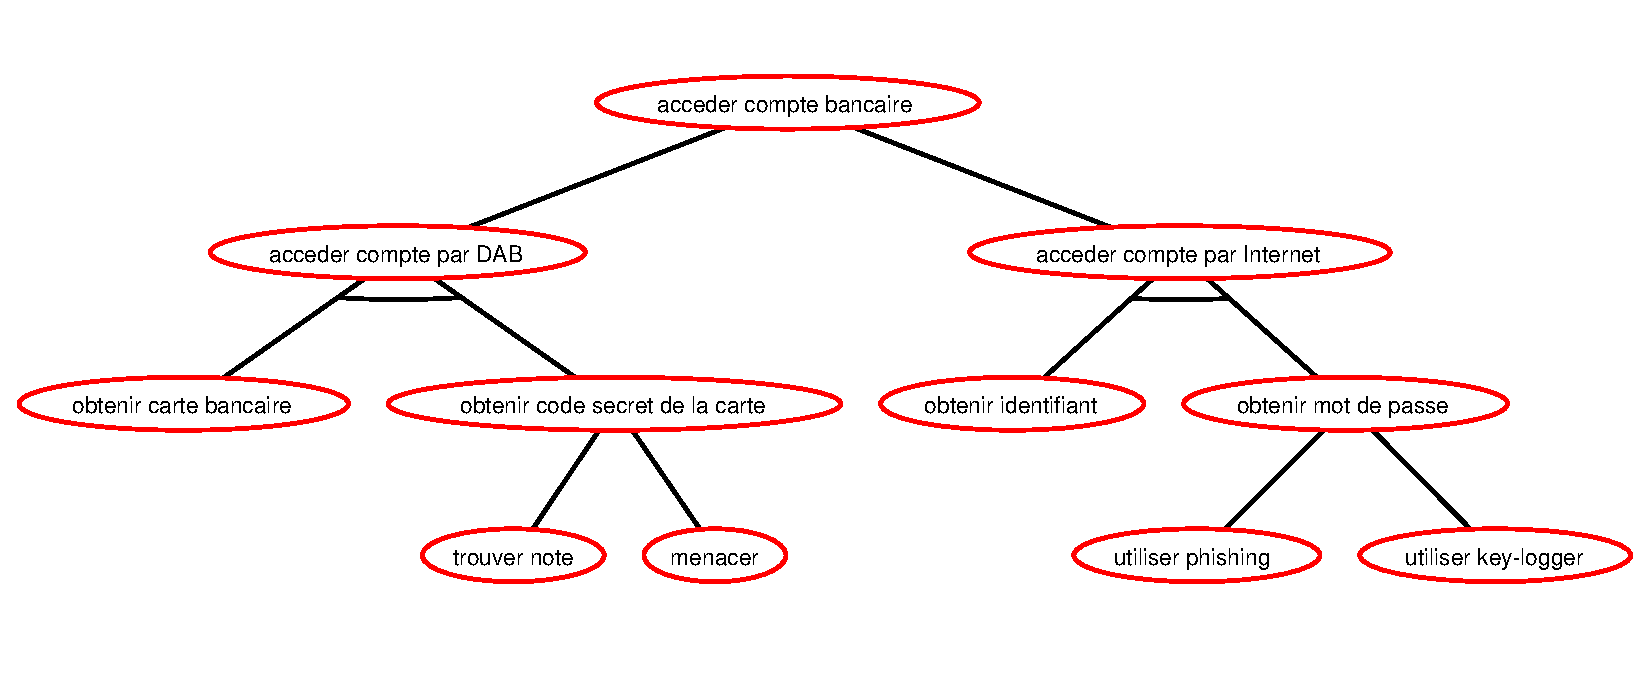
\includegraphics[width=0.8\textwidth]{figure/exemple1_rapport.pdf}
			\end{center}
			\caption{Exemple d'arbre d'attaques}
			\label{fig:arbre_exemple_1}
		\end{figure}

		Depuis 1999, le concept a évolué grâce à la contribution de personnes ayant étendu et amélioré le concept de Schneier. Ces personnes ont en particulier étendu le concept d'arbre d'attaque à celui d'arbre d'attaques et de défenses, aussi appelé Attack-Defense-Tree (ADTree), où sont également représentés les défenses mises en place et que le potentiel attaquant aura besoin de désactiver pour atteindre son but. Les défenses sont traditionnellement représentés par des rectangles. Le même cas que précédemment pour lequel des défense auraient été mises en place pourrait correspondre à la Figure \ref{fig:arbre_exemple_2} : Pour accéder au compte l'attaquant à besoin de désactiver l'authentificateur, même en possession du login ET du mot de passe

        \begin{figure}
            \begin{center}
                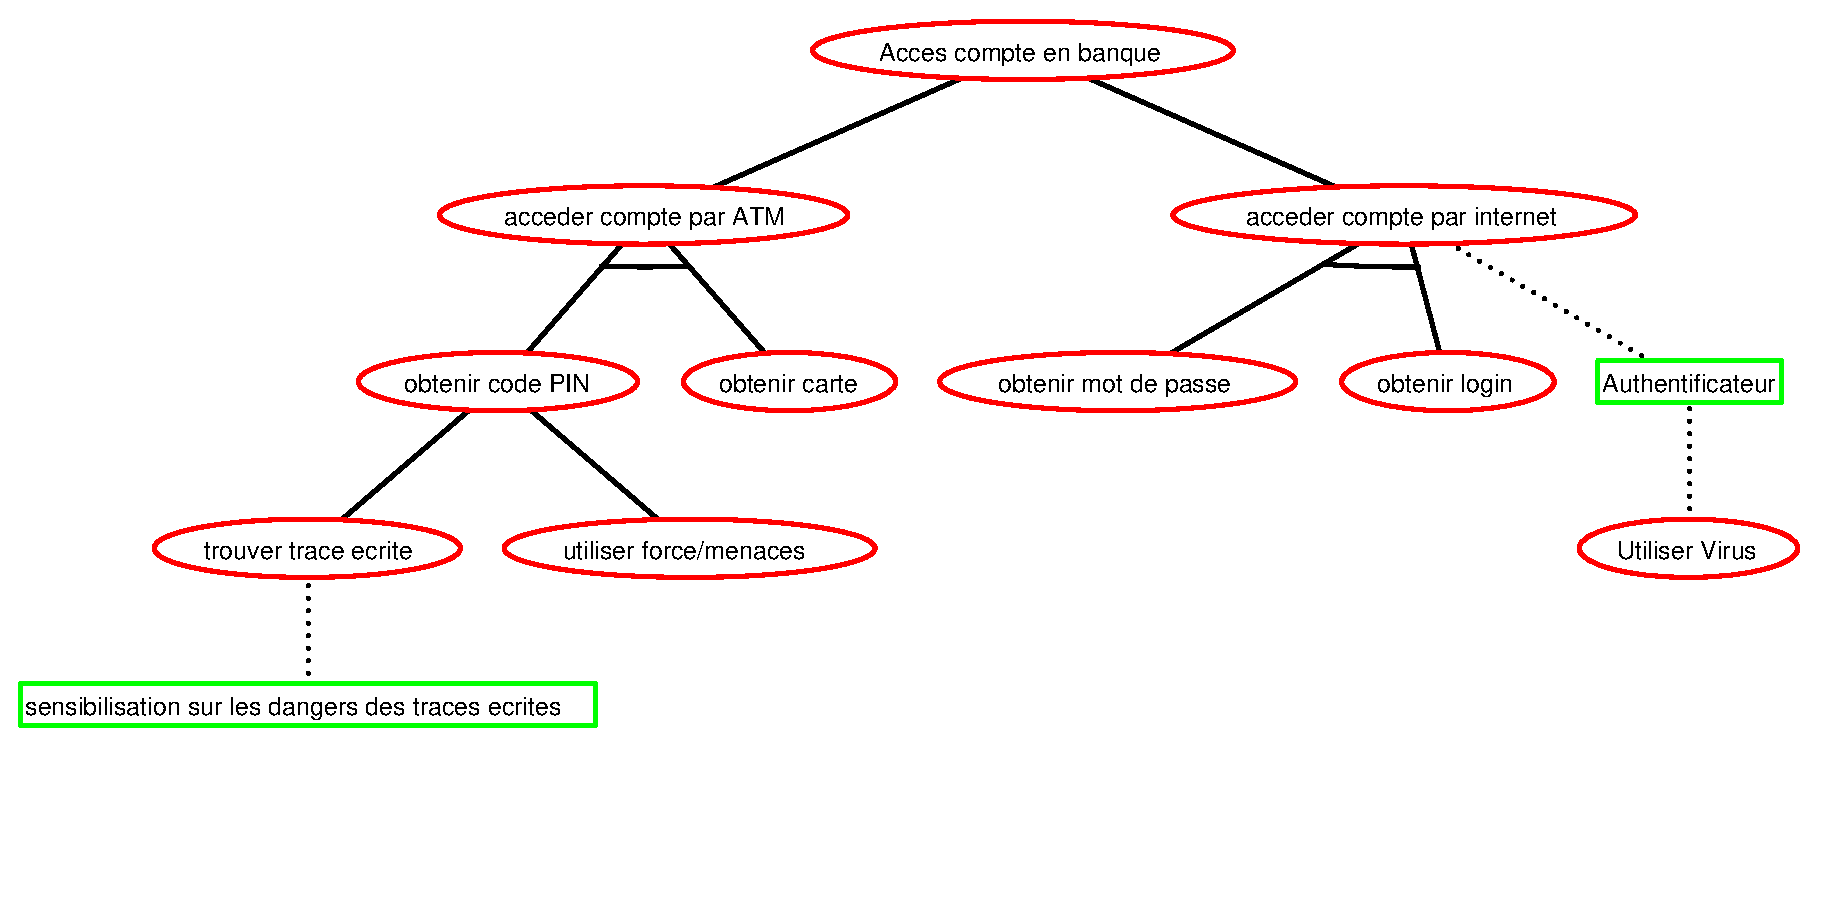
\includegraphics[width=1\textwidth]{figure/exemple2_rapport.pdf}
            \end{center}
            \caption{ADTree}
            \label{fig:arbre_exemple_2}
        \end{figure}

	\subsection{Implémentations des ADTree}
		Plusieurs logiciels implémentant le concept des arbres d'attaques ou des ADTree ont été développés.
        
        \subsubsection{Logiciels propriétaires}
            \paragraph{SecurlTree} Logiciel de création et d'analyse d'arbres d'attaques développé par la société Amenaza

            \paragraph{ATTACKTREE+} logiciel de création et d'analyse d'arbres d'attaques développé par la société Isograph
        
        \subsubsection{Logiciels Open-Source}
            \paragraph{ADTool} Logiciel développé par une équipe de chercheur de l'université du Luxembourg pour la modélisation d'ADTrees (le logiciel avec lequel nous allons travailler)

        \subsubsection{Synthèse}
            Aujourd'hui, les arbres d'attaques tels qu'introduits par Schneier sont utilisés par de nombreuses entreprises. Ceci est dû à l'avantage de pouvoir partir du point de vu de l'attaquant et donc de concentrer les efforts de défenses là où ils seront le plus utiles, à l'inverses d'un certain nombres d'autres stratégies de défense qui vont se concentrer seulement sur la défense du point de vue du défenseur (par exemple les arbres de défaillance), aboutissant forcement à une estimation des dangers incomplète. 

            Cela dit, un grand nombre de ces entreprises développent en interne leur propre logiciel de construction et d'analyse des arbres d'attaque/défense sans toutefois utiliser ceux présent sur le marché. En effet, les solutions logicielles ne bénéficient pas d'une grande visibilité, peuvent être chères et ne sont pas forcement faciles à mettre en place. De plus, le nombre de logiciels implémentant les ADTree est assez réduit en comparaison de ceux implémentant les arbres d'attaques. 

            Ceci étant, le développement peut être laborieux même en utilisant un logiciel dédié comme ADTool pour plusieurs raisons : le logiciel n’intègre pas d'arbres génériques ce qui rallonge le développement et oblige de modéliser plusieurs fois la même partie d'arbre, ne permet pas non plus de gérer la quantification de manière dynamique selon qui est l'attaquant, etc.

            Un grand nombre d'amélioration est donc possible : Ce qui nous amène au cahier des charges.
    
    \section{Cahier des charges}
    % Preciser utilisateur
    % Connais deja concept arbre d'attaque
    % Responsable securite d'une entite
    % Preciser des l'intro

    % Structure reflete niveau importance

    En plus de réaliser l'étude de la sécurité du réseau STAR, un autre objectif de ce projet est de réaliser un outil permettant à un utilisateur (potentiellement novice) d'effectuer une analyse sur la sécurité de son système, quelle qu'en soit sa nature\footnote{L'analyse du réseau STAR nous servira donc essentiellement d'exemple pour réaliser notre second objectif.}. Cette analyse devra ensuite lui permettre de mettre en place les défenses les plus adaptées et les plus "rentables"\footnote{Rentable en fonction du critère choisi: coût pour l'attaquant, temps pour l'attaquant, difficulté nécessaire pour mener l'attaque, etc.}, jusqu'à obtention d'un système dont la sécurité le satisfait pleinement.
    
    L'analyse reposera grandement sur l'utilisation d'arbres d'attaque--défense, mais nécessitera une expertise qui ne pourra pas être fournie par le logiciel afin d'être capable de valuer les feuilles des arbres\footnote{C'est d'ailleurs cette étape qui risque de poser le plus de difficultés à un utilisateur novice.}.
    
    Les différentes fonctionnalités requises pour notre logiciel sont listées ci dessous.
    \begin{itemize}
        \item Une bibliothèque de modèles d'attaques existantes (détaillé dans la sous-section \ref{subsec:biblio_atk}).
        \item Un guide (plus ou moins interactif) pour guider l'analyse, même pour un utilisateur novice (sous-section \ref{subsec:guide_inter}). % Reformuler, répétition
        \item Un éditeur d'arbres (sous-section \ref{subsec:edit_arbre}).
        \item Un outil permettant d'alterner facilement entre différents types de comparaison / valuation / fautquejetrouvelemot.
    \end{itemize}

    \subsection{Spécifications générales}
        \label{subsec:spec_gen}
        L'analyse de l'utilisateur sera sauvegardée sous forme de projet. Lorsque l'utilisateur voudra faire l'analyse d'un nouveau système, il devra créer un nouveau projet, et répondre à une série de questions, comme par exemple le type du système ou l'attaquant envisagé (en précisant ses moyens à disposition).
        
        Ces informations permettront de présélectionner des modèles plus pertinents au cas de l'utilisateur, et pourront par exemple servir à générer un arbre de base. L'utilisateur pourrait alors l'éditer pour obtenir un arbre d'attaque correspondant à sa situation.

        % Vérifier ce que je raconte.
        La valuation des valeurs est déjà prise en charge par ADTool. Toutefois, elle ne permet pas de changer aisément de "type" de valuation. Le projet devrait donc stocker les valeurs des arbres, et pouvoir permettre de changer facilement de valuation (passer du coût financier au temps requis, par exemple).
    
    \subsection{Architecture}
        Nous avons décidé de partir sur une architecture modulaire, où une application mère, qui servira de chef d'orchestre, sera chargé de lancer les différents composants, chacun spécifique à une tache en particulier. % Trop long, reformuler.
        Un ébauche de l'architecture envisagée est disponible figure \ref{fig:archi}.

        % Putain c'est moche
        \begin{figure}
            \begin{center}
                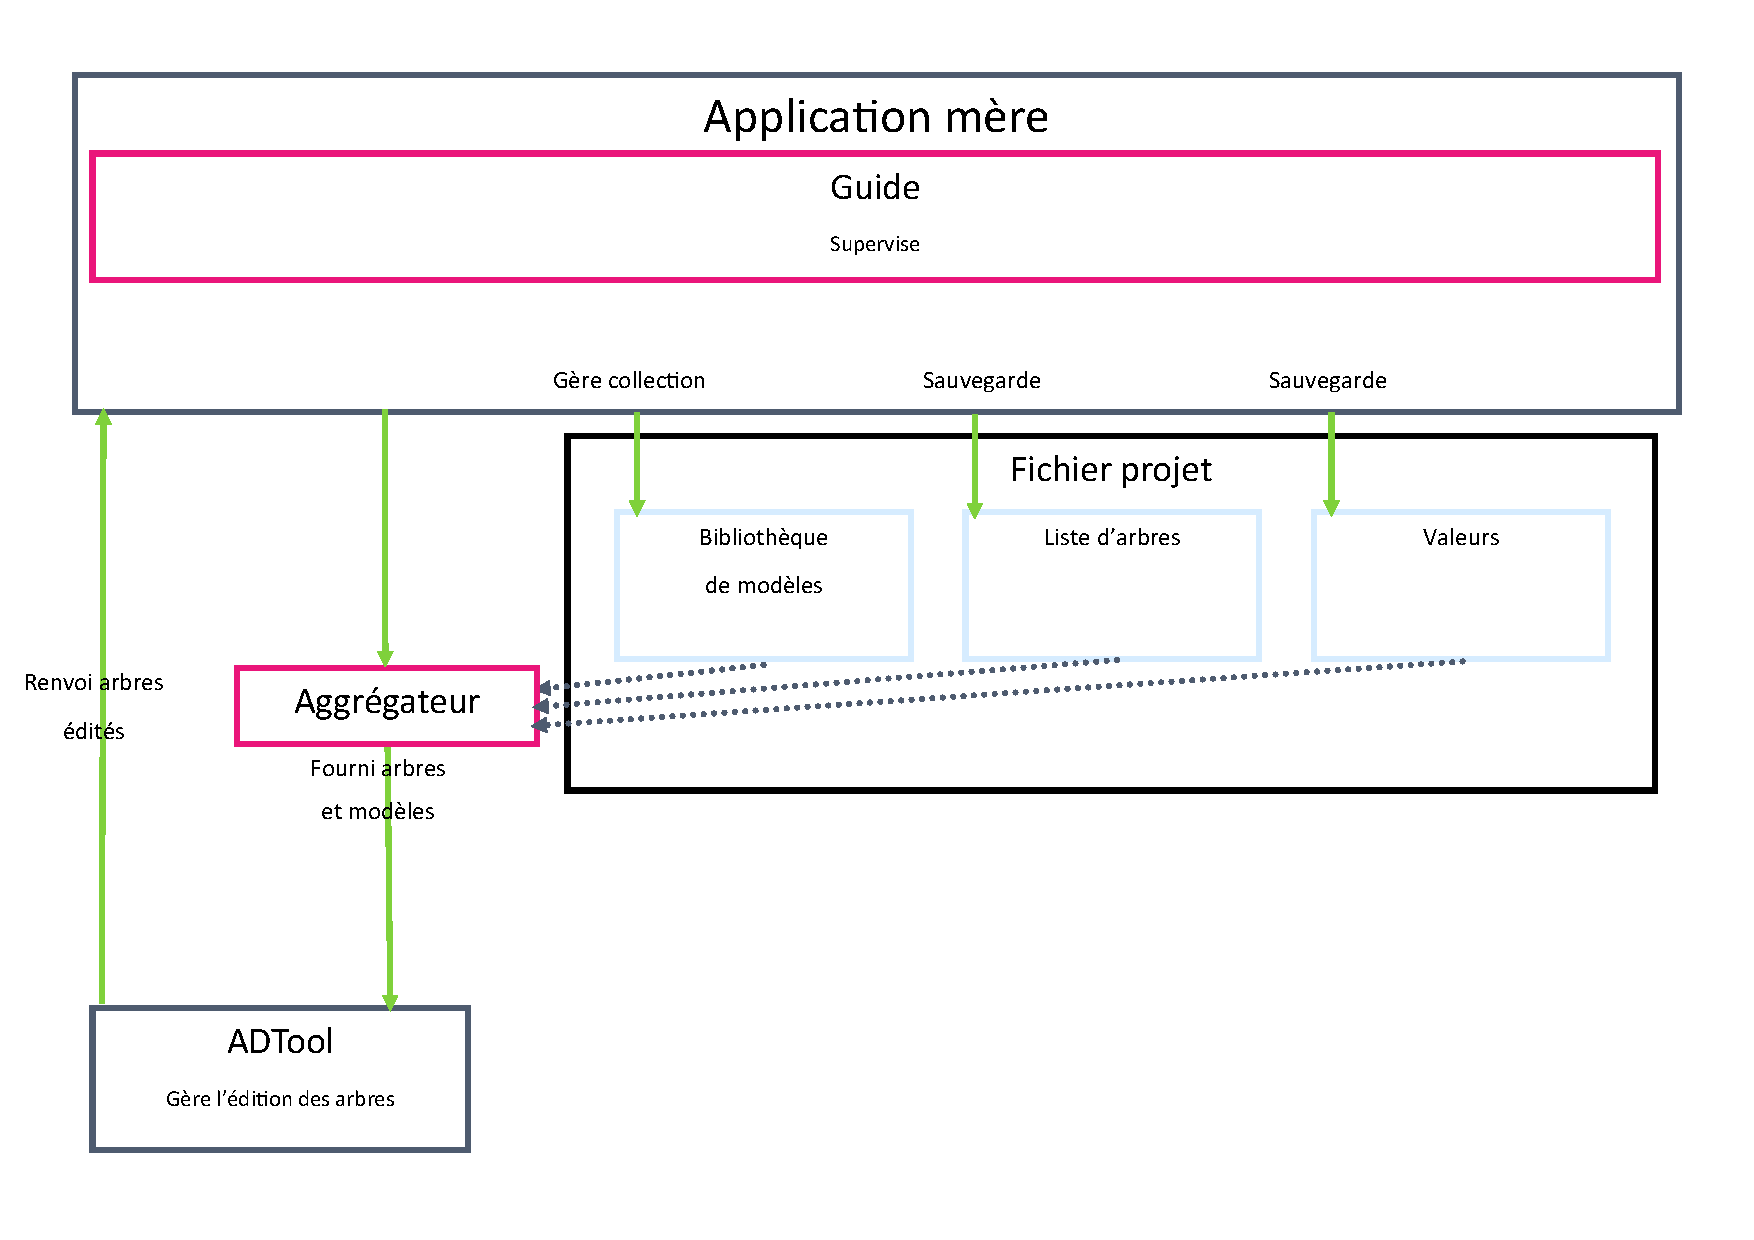
\includegraphics[width=1\textwidth]{figure/archi.pdf}
            \end{center}
            \caption{Différents composants interviendront pour éditer le fichier projet.}
            \label{fig:archi}
        \end{figure}

        % Reformuler ce merdier
        La spécialisation des composants nous permettra d’obtenir une architecture logicielle plus propre, qui facilitera le développement: chaque partie sera indépendante des autres, et les choix techniques de l'une ne limiteront pas une autre.

        Avec ce choix d'architecture modulaire, nous réaliserons donc plusieurs outils spécialisés, mais qui le feront bien, plutôt que faire une seule grosse application qui fera tout de manière médiocre et dont l'architecture rendra toute modification très difficile.
        
        De plus, cette architecture peut potentiellement nous permettre de réutiliser certains outils dans d'autres contextes, ou encore de remplacer un des logiciel par un autre sans trop de difficulté. 
    
    \subsection{Bibliothèque d'attaques}  
        \label{subsec:biblio_atk}
        La bibliothèque d'attaques servirait à décrire des cas très généraux, que l'utilisateur pourrait détailler en fonction de sa situation. 
        
        % En fait on s'en fout ?
        Afin de garder les choses lisibles et ne pas surcharger les autres projets, chaque projet stockera sa propre bibliothèque. De plus, cela rendra la copie de projets entre différents ordinateurs plus aisée.
        
        La bibliothèque d'attaques du projet sera préchargée de diverses attaques en fonction des réponses de l'utilisateur lors de la création du projet, et pourra par la suite être complétée (ou épurée, c'est tout comme) en ajoutant des modèles de base (livrés avec notre application) ou venant d'autres sources (comme Internet, par exemple).
        
        Dans notre exemple (la STAR), nous pourrons fournir des arbres d'attaque de réseaux de transport communs à toutes les villes de France, que nous pourront ensuite détailler pour la ville de Rennes.
      
    \subsection{Guide interactif}
        \label{subsec:guide_inter}
        % Mieux definir
        % Dire qu'on laisse ouvert
        % Reformuler
        Le guide doit être capable d'expliquer à l'utilisateur comment faire son analyse. Celle ci sera découpée en plusieurs étapes (en fonction d'une méthode générique que nous auront précédemment présélectionnée). % Insérer référence ici

        Son niveau de verbosité pourra être adapté en fonction de l'expertise de l'utilisateur, allant par exemple de novice à expert. % Supprimer répétition.
        
        Il pourra par exemple poser une série de questions à l'utilisateur, afin de générer un arbre dit "de base" sur lequel l'utilisateur pourra commencer son analyse.
        
        Chaque notion devra être expliquée de manière claire et concise.

        % Ouais, non.
        Nous pensions faire référence au célèbre trombone magique de Microsoft Office, mais, pour des raisons de droit, nous utiliseront à la place une agrafeuse.
        
    \subsection{\'Editeur d'arbres}
        \label{subsec:edit_arbre}
        Pour l'édition des arbres, nous utiliserons un outil préexistant, à savoir AD Tool~\cite{adtool_paper}.
        
        Toutefois, afin de rendre l'édition des arbres plus simple et plus fluide, nous rajouterons quelques fonctionnalités. Celles ci seront pour la plupart en rapport à l'import/export d'arbres.

        L'objectif en effet serait de faire générer un arbre par notre application mère à partir de différents modèles, pour ensuite demander à l'utilisateur de réaliser les finitions.
    
    \subsection{Multiplate-forme}
        Nous allons dans un premier temps nous concentrer sur une seule plate-forme, à savoir Microsoft Windows. Ainsi, nous n'auront pas à gérer les difficultés de l'écriture de programmes multiplate-formes, nous laissant le champ libre pour nous occuper uniquement des fonctionnalités de notre application.

        Toutefois, afin de ne pas tuer dans l’œuf un éventuel portage ultérieur, nous nous éforcerons de choisir des technologies disponibles pour tout les systèmes d'exploitation, afin de minimiser le travail nécessaire.

    \subsection{Synthèse}
        Faire une liste
    
    \section{Outils}
    \label{sec:outils}
    	
		Nous avons choisis d'employer des outils répondant au mieux à notre cahier des charges tout en s'intégrant bien à notre formation.  Ces différents outils sont décrits ci-après.
    	
    \subsection{ADTool}
    	Comme mentionné dans la section \ref{sec:cahier}, ADTool fera partie intégrante de notre logiciel. En effet, ADTool est libre et son développement a nécessité un travail conséquent. Il est donc pertinent de ne pas développer notre propre éditeur et afficheur d'ADTrees, mais plutôt d'utiliser ADTool pour qu'il remplisse ces fonctions.
    
         
    \subsection{Outils de gestion de projet}
        Pour permettre le versionnement de notre projet, nous avons choisi d'utiliser {\bf Git} \footnote{https://github.com} pour son efficacité et sa simplicité d'utilisation. De plus, il semble s'imposer progressivement dans le monde professionnel, au détriment de Subversion.
        
        Pour le partage de fichiers lourds, la rédaction de notes de réunion, ou plus simplement pour mettre rapidement des idées en commun, nous avons décidé d'utiliser {\bf Google Drive}, que nous préférons à Dropbox, car ce dernier ne permet pas d'écrire simultanément sur un même document.

        Enfin, il nous est demandé d'employer {\bf MS Project} comme outil de planification, que nous utiliserons donc pour tenir à jour le planning du projet.

	\subsection{Systèmes d'exploitation}
	   Comme mentionné précédemment, nous développerons notre application pour {\bf Windows}, en raison de sa très grande présence dans les entreprises. Nous souhaitons cependant garder la porte ouverte à une compatibilité avec Linux et Macintosh, au cas où un futur portage serait envisagé. Ces considérations nous ont amenés à choisir les langages de programmation décrits ci-après.
	
    \subsection{Langages de programmation et environnements de développement intégrés}
        Pour notre application, l'emploi du {\bf C++} nous parait pertinent. Bien que, de par sa nature, Java permette une compatibilité sur tous les systèmes d'exploitation, nous souhaitons éviter d'utiliser ce langage sur la totalité du projet. En effet, le C++ étant très répandu en entreprise, nous souhaitons nous y confronter. De plus, tant que nous utilisons des librairies standardisée, un portage sur Linux ou Macintosh reste possible. Par conséquent, nous utiliserons {\bf Visual Studio} pour développer en C++, car c'est l'environnement de développement intégré actuellement le plus puissant et le plus utilisé  pour ce langage.
        
        Enfin, pour les améliorations apportées à ADTool --- qui est écrit en Java --- nous emploierons {\bf IntelliJ IDEA}.

    \subsection{Interfaces graphiques}
        L'interface graphique de notre suite est primordiale pour garantir une certaine ergonomie à l'utilisateur. Toujours dans un souci de compatibilité, notre choix s'est porté sur {\bf Qt} pour l'interface que présenteront les logiciels de notre suite --- autre que ADTool. 
        
        Pour ce dernier, nous considérons que le logiciel est déjà suffisamment simple et intuitif, et qu'y apporter des améliorations graphiques demanderait une charge de travail élevée pour une amélioration minime. Par conséquent, nous ne prévoyons pas de modification de son interface.

    
    \section{Organisation du projet}
	\subsection{Répartitions des rôles}
	    Étant donné que trois membres du groupe partent à l'étranger au second semestre, nous avons fixé une organisation précise pour que le projet se déroule de la meilleure manière possible. Les différents rôles ainsi décidés au sein du groupe sont décrits ci-dessous.
	    
	    \paragraph{Coordinateur} Le coordinateur s'occupe de planifier les réunions de projet et de les animer. Il est le contact privilégié des encadrants. Son rôle est aussi de s'assurer de l'avancée des rapports et de leur relecture. Il changera régulièrement afin que tout le groupe assure ce rôle. Hoel {\sc Kervadec} est le premier coordinateur jusqu'à la livraison de ce rapport. Corentin {\sc Nicole} sera le prochain coordinateur, puis Florent {\sc Mallard} assurera ce rôle. De cette manière, chacun des étudiants partant en études à l'étranger aura tenu la place de coordinateur avant son départ.
	    
	    \paragraph{Administrateur système} L'administrateur système s'occupe de maintenir à jour les plates-formes et outils utilisés durant le projet (GitHub, GoogleDrive, etc.). Valentin {\sc Esmieu} est en charge de ces plates-formes.
	    
	    \paragraph{Scribe} Un scribe est volontaire à chaque début de réunion afin de prendre des notes. Ce rôle est communément assuré par les personnes disposant de leur ordinateur à l'{\sc Insa} afin de rédiger un compte-rendu en direct sur le Google Drive.
	    
	    \paragraph{Responsable planification} Le responsable planification est en charge du suivi et de la mise à jour de la planification du projet. Celui-ci utilisera le logiciel MS Project, comme indiqué dans la Section \ref{sec:outils}.
	    
	    \paragraph{Décompte du temps} Au sein du groupe, le décompte du temps passé sur le projet se fait de manière autonome. Nous utilisons pour cela un tableur créé sur Google Drive. Le coordinateur et le responsable planification consulteront ce tableur afin d'effectuer au mieux la répartition des tâches restantes.

	    Nous avons également décidé de nous réunir de manière hebdomadaire le mercredi soir. Au cours de ces réunions, nous nous concertons sur les tâches à réaliser, et les répartissons entre nous. C'est aussi à ce moment que nous débattons sur les principales questions qui seront posées au cours de la prochaine réunion avec nos encadrants.

	    
	\subsection{Planification}
		
		En septembre, nous avons suivi des cours sur les ADTrees afin de se familiariser avec le concept, puis nous avons découvert ADTool et son fonctionnement. Nous avons ensuite jugé utile de suivre un cours de cryptographie afin de mieux saisir les protocoles de communication sécurisée. Gildas {\sc Avoine} nous a donc dispensé un cours de deux heures sur notre temps libre. Ceci nous a permis d'appréhender les concepts de protection des cartes Korrigo. Ceux-ci pourraient nous être utiles pour analyser et valuer les risques liés à ce type de carte.
		
		Puis, en octobre, nous avons réalisé l'étude de l'existant sur le sujet de notre projet. Puis nous avons élaboré notre cahier des charges et défini l'architecture de notre logiciel. Enfin, nous nous sommes attelés à la rédaction de ce rapport de pré-étude. Comme nous avons noté le temps passé à travailler sur ce rapport, nous pouvons en déduire approximativement le temps qu'il nous faudra pour livrer les suivants. Pour rendre un rapport de vingt pages, nous avons passé, entre rédaction et correction, environ vingt-cinq heures chacun.
		
		Pour la suite, bien que la planification ne soit pas encore totalement établie, nous pouvons déjà en donner les principaux axes. 

		En novembre, nous allons définir les spécifications fonctionnelles de notre logiciel afin de préciser davantage les différentes interactions entre les modules présents. Nous nous réunirons pour détailler l'interface graphique, puis nous nous mettrons d'accord sur la répartition des tâches et la manière d'implémenter les améliorations d'ADTool.

		Ensuite, jusqu'aux vacances de Noël, nous établirons la planification complète du projet. Elle sera plus détaillée et contiendra un diagramme de Gantt expliquant la répartition des différentes tâches entreprises et leur ordonnancement. À ce moment, nous aurons donc tous les outils nécessaires à la modélisation de notre projet. Au terme de cette échéance, nous serons en mesure de présenter notre planification ainsi que nos spécifications lors des soutenances des 18 et 19 décembre.

		De début 2015 à mi-février, nous définirons l'architecture interne de notre logiciel, et nous pourrons en parallèle commencer l'implémentation. Suivra enfin le développement complet de notre logiciel, jusqu'à la fin de l'année scolaire. Enfin, nous présenterons le projet complet durant les soutenances des 28 et 29 mai.

	    

    
    \section{Risques}
    Nous pouvons d'ores et déjà envisager des situations dans lesquelles nous ne serions pas en mesure de livrer le projet dans l'état que nous avions prévu en ce début d'année scolaire.
    Le facteur principal est bien entendu humain. En effet, la moitié du groupe partant étudier à l'étranger dans le cadre de la mobilité internationale, il se peut que nous ayons légèrement sur-estimé nos capacités de travail et annoncé une tâche trop difficile à exécuter. De plus, sur les trois personnes restant en France, une incapacité à travailler sur le projet, quelle qu'elle soit, aurait des répercussions sur l'avancée globale du livrable. Mais une incapacité de ce type serait accidentelle et très peu probable.
    
    Des problèmes d'ordre technique peuvent également survenir. Il est ainsi possible que nous rencontrions des difficultés à mettre en place la chaîne logicielle prévue, la plupart d'entre nous n'en ayant jamais développé. Nous pourrions ainsi connaître des problèmes dans la communication des différents composants de la chaîne logicielle. Il faudra, pour éviter cela, bien choisir les langages utilisés dans la conception logicielle.
    Une perte de données stockées sur Git, ou bien de fauses manipulations entrainant une perte de données totale ou partielle ralentirait \textit{a minima} le projet, et dans le pire des cas le rendrait impossible à livrer tel que nous l'avons promis. Cependant, Git est équipé d'outils de récupération pour les \textit{commit}, et le projet sera normalement mis à jour (\textit{pull}) sur chacun de nos ordinateurs personnels, réduisant quasimment ce risque à zéro.



    % a eviter
    \nocite{*}

    \bibliographystyle{plain}
    \bibliography{input/biblio}

    % Manoucherie incoming
    \pagevierge
    \ifthenelse{\isodd{\thepage}}
    {\pagevierge}
    {}
    
\includepdf[pages=2]{figure/couv.pdf}
\end{document}